\section{Loop-Free}
\label{sec:example}

\begin{figure}[t!]
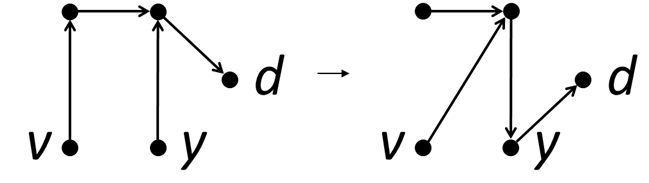
\includegraphics[width=3in]{figures/noloops.png}
\caption{something}
\end{figure}

\subsection{Example}

Applying routing updates in a way that guarantees no loops is a basic but already interesting consistency property. Consider the five node example network in Figure TODOnoloops. The existing routing to destination $d$ on the left of the figure should be updated according to the right of the figure. A naive way to update is to simply send out the forwarding updates (e.g., ``node $u$: for destination $d$ send to $x$''). However, when doing so, it might happen that node $x$ updates its rule before node $y$, introducing a routing loop between nodes $x$ and $y$. This loop will eventually disappear, namely once node $y$ updates its rule, but in an asynchronous system it is difficult to give guarantees when this will happen.

At the other end of the spectrum, the SDN controller could first (i) distribute the new rules, then (ii) wait for an acknowledgement of all the nodes that they have received the new rules, then (iii) tell all the nodes to stop sending packets, and finally, once (iv) they all acknowledged that, (v) tell the nodes to now use the new rules. After the nodes (vi) acknowledge that they are using the new rules, the SDN controller can tell them to (vii) remove the old rules, as they are not needed anymore. This solution does not suffer from loops, as the old and the new solution are well-separated in time.\footnote{Strictly speaking, this protocol is not sufficient, as there might be packets in transit, still using the old rules when rushing through the protocol. Consider a packet sent from sent from $y$ to $x$ shortly before $y$ received the order to stop sending (iii). If node $x$ already passed the last step of the protocol when receiving the packet, node $x$ has not other option then sending the packet back to node $y$, i.e. the packet is experiencing a loop.} However, it is also terribly slow. One may speed up the process by omitting steps (iii) and (iv). Now, assuming that node $x$ received the command to use the new rule (v) earlier than node $y$. As such, in order to guarantee no loop between nodes $x$ and $y$, we must introduce version numbers in packets such that nodes $x$ and $y$ know that packets from $x$ respectively $y$ must be treated according to the new respectively old rules. This is the solution proposed by \ref{theoriginalprincetonpaper}.

One may ask whether version numbers are really necessary, just to guarantee no loops? Also, one may ask whether a faster solution is possible. What nodes are really dependent on each other? This may look like a technicality, but as we all know, nodes are often temporarily unavailable or reacting slowly. If a node must wait for another node, there should better be a consistency reason for it, and not merely protocol overhead. Is there something like a \emph{minimal protocol for a given consistency guarantee}? This is exactly the question we address in this paper.

Regarding our example, the answer to this question is quite simple. Node $u$ does not even need to change its rule, as it always just forwards to $x$, hence node $u$ does not even have to be informed about the rule changes. Node $v$ can switch immediately after being informed about the new rule, as no matter whether using the old or new rule, the packet will always end up at node $x$, with no possibility to experience a loop. Also node $y$ can switch immediately to the new rule, as its packet will then directly reach the destination node $d$. The only critical node in our example is node $x$, for which we understand that node $x$ must wait until node $y$ implemented the switch, as otherwise our network might experience a loop.

More generally, as we will see (TODO: later OR in the remainder of this section), achieving loop-free consistency requires rule updates to wait for each other in a \emph{dependency forest}, i.e., a node may have to wait for one parent node having switched to the new rule before being able to switch itself. We will show two solutions, one with advantages regarding practice as the parent in the dependency forest is always a neighbor node. The practical solution is provably fast, however, it is not optimal regarding dependencies. So, in addition, we also show a more theoretical solution, which (in polynomial time) can compute the minimal dependency forest, i.e. where nodes can switch to the new solution in minimal time.

\subsection{Practical Protocol}

The minimal protocol below will have dependencies between nodes that are not neighbors in the network. In the simple practical protocol described here, any parent in the dependency forest is also a neighbor in the network, which simplifies signaling. A node is a root of the dependency forest, if the node does not have to update its rule. In our example, the destination $d$ and node $u$ are roots. A node $p$ is a parent of a child node $c$ in the dependency forest if $c$ points to $p$ according to the new rules, e.g. $d$ is a parent of $y$, which is a parent of $x$, which in turn is a parent of $v$. Now, starting at the roots, nodes first switch to the new rule, and then inform all their children in the dependency forest to switch as well.

Apart from the packets-in-transit problem described above, correctness is immediate: Nodes that are in the dependency tree of the destination will only switch to the new rule once all the nodes on the new path to the destination have already switched. (TODO: what about that trick to cut the dependency tree into forests as node which are static? One could also describe the even simpler solution, and then mention this as an improvement...? Ratul?)

Based on the discussion on the example, it is easy to see that this solution is not minimal, as node $v$ cannot switch immediately, after learning the new rule.

\subsection{Minimal Protocol}

As in the practical protocol, we construct a dependency forest, and parents will inform their children when it is safe to use the new rule. The only difference is that the dependency forest is cut to its bare minimum.

We need to define \emph{good} and \emph{bad} nodes as follows: The destination $d$ is by definition good. All other nodes $u$ are defined as good or bad regarding the node $v$ at the end of the new forwarding rule \texttt{u.new = v}. If all paths (mixing new and [TODO: still valid] old rules) of $v$ point to the same node $r$ (possibly $r = d$), without loop, then $u$ is good. Else ($v$ has a path that points into a loop) $u$ is bad.

[TODO: is there a framework for algorithms? maybe not... text version instead]

The algorithm to construct the dependency forest is as follows: Initially, we let all good nodes to be roots in the dependency forest. Then, iteratively, while not all nodes are processed, we process an arbitrary good node $u$ by removing its old rule. Removing $u$'s old rule might turn other nodes good; if $v$ turns good when processing $u$, then $v$ is a child of $u$ in the dependency forest.

[TODO: here the old psudo-code]

Algorithm:
All good nodes u have no parent in the virtual forest, i.e. u.parent = nil, good nodes are ready to be processed.
While not all nodes are processed
	Process an arbitrary good node u: remove the old pointer u.old
	For all bad nodes v:
		If processing u made v good, then v.parent = u

[TODO: Remark: This also works with more than two trees, i.e. with multiple versions of old trees and one new tree. Should I describe a more direct algorithm, an algorithm that does recognize good and bad without calling the Tarjan loop discovery subroutine? What about the failures? In several versions, what happens if a node just does not ack the changes of old versions? Will it become a leaf?]




